% ISWC 2026 In-Use Track submission
% Target: https://iswc2026.semanticweb.org/#/calls/in-use
%
% ISWC 2026 In-Use Track CFP Key Dates:
%   Abstract submission due:    2 May 2026
%   Full paper submission due:  7 May 2026
%   Rebuttal:                   11 June - 18 June 2026
%   Notifications:              16 July 2026
%   Camera-ready papers due:    6 August 2026
%   Conference:                 27 - 29 October 2026
%   All deadlines 23:59 AoE
%
% Submission details:
%   Max 15 pages (excl. references and "Declaration of use of Generative AI")
%   Format: LNCS (Springer Lecture Notes in Computer Science)
%   Review: single-blind (not anonymous)
%   Submission via EasyChair (abstract pre-submission required)
%   Published: Springer LNCS proceedings
%
% Track Chairs:
%   Ernesto Jimenez-Ruiz, City St George's, University of London, UK
%   Oshani Seneviratne, Rensselaer Polytechnic Institute, USA
%   Contact: iswc2026-in-use@easychair.org
%
% Based on prior SWJ submission, now migrated to LNCS
% Original: extended version of Text2KG ESWC 2023 Workshop paper

\documentclass[runningheads]{llncs}

%% Packages
\usepackage{dcolumn}

%% Definitions
\newcolumntype{d}[1]{D{.}{.}{#1}}

%% Authors LaTex packages and macros
% enable utf-8 chars
\usepackage[utf8]{inputenc}

% according to error message
\usepackage{booktabs}

% render SVG files: https://tex.stackexchange.com/questions/122871/include-svg-images-with-the-svg-package
\usepackage{svg}

% for tables
\usepackage{tabularx}

% source code rendering
\usepackage{minted}

% hyperlinks
\usepackage{hyperref}
\usepackage{url}

% ORCID rendering provided by llncs.cls

% typographical quoting
\newcommand{\tquote}[1]{``#1''}
% footnotelink
\newcommand{\footnotelink}[2]{\href{#1}{#2}\footnote{#1}}
% define some macros/commands
\newcommand{\wdq}[2]{\footnotelink{https://www.wikidata.org/wiki/#2}{#1 (#2)}}
\newcommand{\wdp}[2]{\footnotelink{https://www.wikidata.org/wiki/Property:#2}{#1 (#2)}}

\newcommand{\wdpTable}[2]{\href{https://www.wikidata.org/wiki/Property:#2}{#1 (#2)}}
\newcommand{\wdqTable}[2]{\href{https://www.wikidata.org/wiki/#2}{#1 (#2)}}

%% Article Info


\title{Semantified CEUR-WS in Wikidata}

\author{Wolfgang Fahl\inst{1}\orcidID{0000-0002-0821-6995} \and
Tim Holzheim\inst{1,2}\orcidID{0000-0003-2533-6363} \and
Christoph Lange\inst{1,2}\orcidID{0000-0001-9879-3827} \and
Jerven Bolleman\inst{3}\orcidID{0000-0002-7449-1266} \and
Stefan Decker\inst{1,2}\orcidID{0000-0001-6324-7164}}

\institute{RWTH Aachen University, Computer Science i5, Aachen, Germany \and
Fraunhofer FIT, Sankt Augustin, Germany \and
SIB Swiss Institute of Bioinformatics, Switzerland}

\begin{document}
\maketitle
\begin{abstract}
The CEUR Workshop Proceedings (CEUR-WS) is a non profit publisher for scientific workshop and conference proceedings since 1995. For more than 30 years it has used HTML and PDF as the single point of truth for the needed metadata to be used by indexers such as DBLP and german national library DNB. Scholars have long craved for persistent identifiers for the core entities involved:  event series, event, proceedings, paper, editor, author, institution and publisher with the goal to allow semantic handling and querying with modern tools. 

In this work we show how the semantification is in progress and Wikidata has been used as the core target infrastructure to overcome the obstacles that the change in workflow has been struggling with since the 2015 Sempub challenge.

\end{abstract}
\keywords{Knowledge Graph \and Linked Data \and Metadata Extraction \and Publishing \and Semantic Web \and Wikidata}

\section{Introduction}\label{sec:Introduction}
\begin{figure}
    \centering
    \includesvg[width=\linewidth]{images/CoreEntities.svg}
    \caption{Most relevant entities for scientific publishing}
     \label{fig:core_entities}
\end{figure}

The Traditional publishing workflows handle the metadata of the needed core entities (as shown in Figure~\ref{fig:core_entities}) in an unFAIR way. Findable, Accessible, Interoperable, and Reusable (FAIR) ~\ref{sec:FAIR}, Single Point of Truth (SPoT), and Single Source of Truth (SSoT) principles are having low priority. Therefore the opportunities to collect the metadata during the different lifcecyle stages of an event as shown in table \ref{tab:ScientificEventLifecycle} are missed. For the future of CEUR-WS publishing we envision a metadata first publishing approach. This work shows how the HTML/PDF SSoT of CEUR-WS at the ceur-ws.org domain (SPoT) has been used to create a Knowledge Graph representation of the relevant entities in Wikidata between 2022 and 2026 as a step in this direction.


\begin{table}
\caption{Scientific Event Lifecycle stages}
\label{tab:ScientificEventLifecycle}
\begin{tabular}{ | m{2.5cm} | m{2.5cm} | m{3.5cm} | m{2.5cm} | m{2.5cm} | }
\hline
\textbf{Stage} & \textbf{Stakeholders} & \textbf{Artifacts Created} & \textbf{Format} & \textbf{Responsibility} \\
\hline
Announcement & Organizers, Marketing Team & Promotional materials, websites, notifications & HTML, Email & Organizers \\
\hline
Call for Papers (CfP) & Organizers, Authors, Reviewers & CfP documents, emails, submission portals, responses & PDF, HTML, Email & Organizers \\
\hline
Performing Conference & Organizers, Chairs, Presenters, Attendees & Schedules, presentations, participant lists, recordings & PDF, PPT, HTML, Video & Organizers \\
\hline
Proceedings Publication & Editors, Chairs, Authors& Finalized papers, indexed and archived content & PDF, HTML & Editors, Authors, Chairs \\
\hline
Indexing & Libraries, Indexing Services & Catalog entries, metadata records & MARC, XML, RDF & Publishers, Libraries  \\
\hline
Referencing/Quoting & Academic Community & Citations, references in future works & BibTeX, HTML & Scholars \\

\hline
\end{tabular}
\end{table}

\textbf{Digital Traces of Scientific Events during their lifecyle:} Table~\ref{tab:ScientificEventLifecycle} shows the stages of the scientific event lifecycle that cumulatively create artifacts related to the event.

Moving the responsibility for curating data for relevant entities (see Figure~\ref{fig:core_entities}) to an earlier stage and thus to the event organizers, while semi-automating the process has several benefits. The quality of the data will increase, and its availability will be much earlier, thus influencing FAIRness---e.g., ensuring computer-readable versions of the core entities are available for downstream systems at each step in the lifecycle. Involving a community such as Wikidata in open source style will further enhance the result \footnote{And will create follow-up issues for the single point of truth data to be discussed later}.  

Scientific communication increasingly relies on the use of knowledge graphs, as exemplified by \footnotelink{https://scholar.google.com/}{Google Scholar} and the evolution of Microsoft Academic Graph~\cite{Wang2020} into OpenAlex~\cite{Priem2022}. Legacy systems based on technologies such as MARC~\cite{Ganseman2015}, PICA~\cite{Costers1997}  or XML are also adapting, highlighted by DBLP's adoption of RDF/SPARQL, with the  \footnotelink{https://qlever.cs.uni-freiburg.de/dblp}{QLever DBLP SPARQL endpoint}~\cite{Bast2017} being the most up-to-date.

\subsection{CEUR Workshop Proceedings}
The CEUR Workshop Proceedings (CEUR-WS) publishing platform (https://ceur-ws.org/) was introduced in 1995 as a means of publishing proceedings of scientific workshops (and smaller conferences) in computer science. 

CEUR-WS offers a free online service that provides open access to the published proceedings originally hosted by RWTH Aachen University's Chair for Information Systems and Databases and now moved to Gesellschaft for Informatik in 2026. CEUR-WS is operated by the CEUR-WS Editors -- a team of unpaid volunteers -- working as a de facto non-profit organization. More than 4,200 Volumes containing over 90,000 PDF documents have been published in total until 2026.

Technically, all data and metadata of the proceedings are directly represented using HTML, PDF and a filesystem directory hierarchy, and delivered via the HTTP and FTP protocols. 

CEUR-WS does not use a Content Management System for publishing but relies on pure HTML and PDF for rendering its \footnotelink{https://ceur-ws.org}{public website}. The metadata for these publications is only indirectly available through indexing services such as dblp~\cite{Ley2009} and {K10plus}\cite{k10plus2019}\footnote{\url{https://dblp.org/}, \url{https://opac.k10plus.de}}. Unfortunately both DBLP and k10plus do not have a complete set of metadata records for all volumes as of April 2026 and in both cases there is a delay of some weeks/months before new volumes are picked up for indexing.

There have been multiple attempts in the past to make the metadata of the CEUR-WS platform available for computer based analysis and querying. None of these attempts has been consistent and continuous so far – the CEUR-WS editors workflow still directly creates the HTML artifacts and still ask authors and proceeding editors to work this way as described in the CEUR-WS “how to submit” guide~\cite{CEURHowtoSubmit}.

This work reports on the successful start of the semantification of CEUR-WS with Wikidata as a target knowledge graph with the goal to achieve consistency and continuity for the future. 

The challenge was in handling the textual natural language description parts of the CEUR-WS content that is inherently still part of the semi-digitized approach of using HTML and PDF. We propose to have a better separation of concerns of metadata, display and storage and started implementing it.

\subsection{The Trend towards FAIR Data and Open Science: Semantification}\label{sec:FAIR}
% FAIR Data Introduction - why is this relevant? EOSC, NFDI, Open Access, Open Science
% FAIR Data as a basis for Knowledge Graphs
Since their inception, the FAIR principles~\cite{GOFAIR2019,Wilkinson2016} have been a  success. They have been adopted by various industries (e.g., the pharmaceutical industry) and national and international projects (e.g., the Common European Dataspaces). 
Persistent Identifiers (PIDs) and rich metadata are the core components of the FAIR principles, and they provide the means to create Knowledge Graphs~\cite{Cousijn2021}.

Representing digital traces of scholarly communication in Knowledge Graphs (KGs)~\cite{Hogan_2021} is useful for supporting use cases such as literature search and recommendation of events for attendance or publishing. The metadata of the most relevant entities as outlined in Figure~\ref{fig:core_entities}\footnote{The original SVG (see \texttt{http://cr.bitplan.com}) has clickable links to the Wikidata properties and entity types} need to be made available to offer such a knowledge graph. The the entities at the core of this work are depicted in bold and blue.


The term \tquote{Semantic Web}~\cite{BernersLee2001} has been coined by Tim-Berners Lee et al.\ to describe the effect of resources on the Web interlinked making use of such metadata.
Therefore \tquote{Semantification} was chosen as the title of the project and this paper to describe the process of creating a Knowledge Graph and making the results available in a Semantic Web fashion. The Semantification of CEUR-WS has been attempted multiple times in the past~\cite{Lange2014,Sateli2015} -- always under the assumption that a self-maintained RDF/SPARQL endpoint would be the goal to achieve. The results have not been consistent and durable since the publishing workflow has not been adapted and the single point of truth for the metadata is still buried in the HTML/PDF documents often in pure text sections. The fear of maintenance follow-up problems, given that CEUR-WS is a non-profit service with no budget, was a major obstacle. 

\subsection{Challenges in making CEUR-WS more FAIR via Semantification}\label{sec:fair_challenges}

To semantify CEUR-WS, the following requirements were most relevant:
\begin{itemize}
    \item the metadata should follow the FAIR~\cite{GOFAIR2019,Wilkinson2016} principles 
    \begin{itemize}
    \item \textbf{Findable}
    \begin{itemize}
        \item F1: (Meta)data are assigned globally unique and persistent identifiers (PIDs) (see Section~\ref{sec:event_pids}).
        \item F2: Data are described with rich metadata.
        \item F3: Metadata clearly and explicitly include the identifier of the data they describe.
        \item F4: (Meta)data are registered or indexed in a searchable resource.
    \end{itemize}
    \item \textbf{Accessible}
    \begin{itemize}
        \item A1: (Meta)data are retrievable by their identifier using a standardised communications protocol
        \item A1.1: The protocol is open, free, and universally implementable
        \item A1.2: The protocol allows for an authentication and authorisation procedure, where necessary
        \item A2: Metadata should be accessible even when the data is no longer available
    \end{itemize}
    \item \textbf{Interoperable}
    \begin{itemize}
        \item I1: (Meta)data use a formal, accessible, shared, and broadly applicable language for knowledge representation.
        \item I2: (Meta)data use vocabularies that follow FAIR principles
        \item I3: (Meta)data include qualified references to other (meta)data
    \end{itemize}
    \item \textbf{Reusable}
    \begin{itemize}
        \item R1: (Meta)data are richly described with a plurality of accurate and relevant attributes
        \item R1.1: (Meta)data are released with a clear and accessible data usage license
        \item R1.2: (Meta)data are associated with detailed provenance
        \item R1.3: (Meta)data meet domain-relevant community standards
    \end{itemize}
\end{itemize}

    \item relevant queries should be supported, as derived from the original set of queries of the 2014 Semantic publishing challenge as outlined in Section~\ref{sec:sempub_challenge}
    \item the metadata should reuse an established ontology
    \item the manual and automatic curation of entries should be possible with public access for all stakeholders, e.g., editors, authors, organizers, publishers, indexers
    \item the infrastructure should be stable and there should be sufficient trust in its long term availability
    \item an open source non-profit infrastructure is preferred since this is also the mode of operation of CEUR-WS
\end{itemize}

Given the HTML/PDF/text input of CEUR-WS, the corresponding Knowledge Graph needs to be created and the single-point-of-truth computer readable metadata be separated from the different representations such as HTML so that the above requirements are fulfilled. 

%The \footnotelink{https://cr.bitplan.com/index.php/Semantic\_Publishing\_Challenge}{original task} called for 20 such queries to be answerable. 
%Formally we need to implement a function hat takes two Trees (IT,PT) as an Input and outputs a Graph G=(V,E).

%The IT Tree is the HTML Dom Tree of the CEUR-WS index page where the leaves are HTML markup nodes that might be annotated with an attempted RDFa syntax. 

%The PT Tree is a three level filesystem /HTML Dom tree of 
%Directories per volumes - with an index HTML DOM Tree for the volume and a list of individual PDF files per paper of the volume.

%The leaf node contents are the PDF contents of the files and the HTML markup nodes of the Volume index page.
Both the HTML and PDF encoding of the original scientific content are structured for the purpose of optimizing the display / output on paper or screens; therefore, there is a structure loss compared to what was originally available in the text document processor files that the authors might have been using~\cite{Fahl2023}. Figure~\ref{fig:digital_publishing} shows the part of the publishing process where the rendering step causes this loss. Most scholars are not aware of this loss in the daily use of published content just because the documents are optimized for display and human consumption~\cite{Yu2020}. For the metadata extraction and use in knowledge graphs the difference is sometimes disastrous, e.g., when a simple text from a PDF document can not be extracted any more due to exotic styling and formatting or simply because only a scanned graphic image version of an older document is available that needs optical character recognition to extract the textual content see table~\ref{tab:format_comparisons}.  

\begin{figure}
    \centering
    %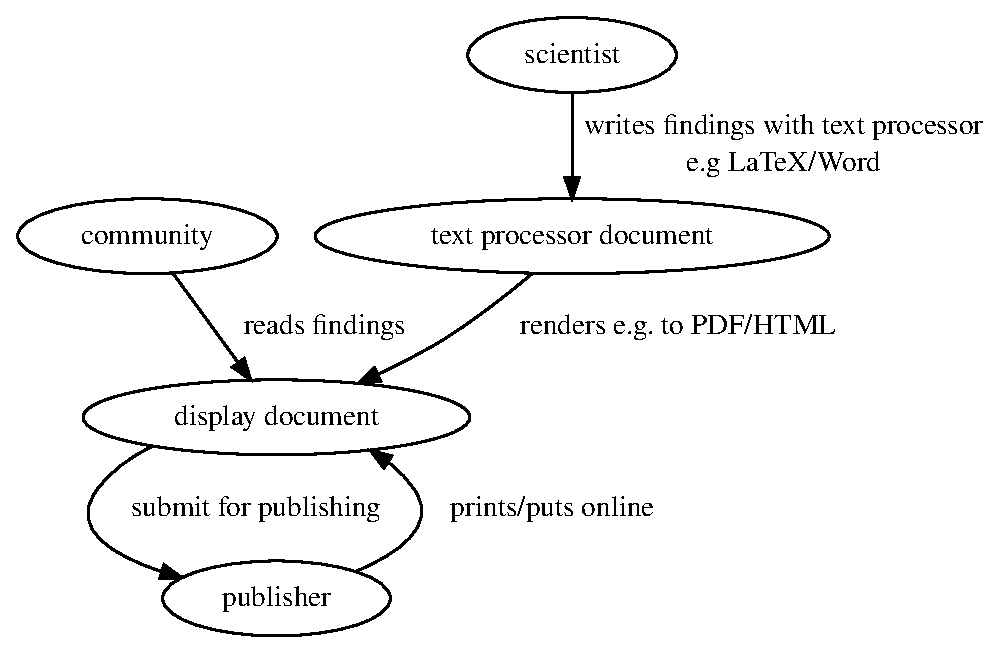
\includegraphics[width=0.7\linewidth]{images/DigitalScientificPublishing.eps}
    \includesvg[scale=0.6]{images/DigitalScientificPublishing.svg}
    \caption{Text processing step of digital Scientific Publishing}
     \label{fig:digital_publishing}
\end{figure}

The metadata needed for creating the knowledge graph is only available in natural language/text form and follows rules that have been changed multiple times during the history of CEUR-WS. From 2013 to 2026, there have been 33 different versions of the index file template with no proper tracing of what was changed from version to version. The index and volume HTML files were often edited manually, leading to minor, undocumented differences even within these versions. The usage of the different page versions follows a long-tail Zipfian distribution with 5 versions covering 60\% of all volumes. 

% https://cr.bitplan.com/index.php/CEUR-WS_Versions
\subsection{Contributions of this Paper}
The core contributions presented in this work are:
\begin{enumerate}
    \item To provide the tools, infrastructure and approaches to modify the CEUR-WS publication workflow to consistently supply high quality FAIR metadata (Semantification). Tools such as CEUR-WS Volume Browser, Semantic MediaWiki, and Single Point of Truth Server are detailed in section~\ref{sec:implementations_and_demos}. 

    \item Splitting the metadata for the three main entities Event, Event Series and Proceedings as a major step towards improving the metadata quality, e.g., by allowing event series data to be checked for completeness and be completed from different sources where possible. Unfortunately, currently none of the stakeholders have shown enough motivation to do this completion, while it is valuable, e.g., for assessing the quality of an event series. The necessary change of perspective to convince the stakeholders is a chicken-egg problem, which the CEUR-WS semantification will help to facilitate. 

    \item Providing a bootstrapping~\cite{Bardini2001,Engelbart2007} approach to get rid of manual editing of the CEUR-WS website content and instead using a CMS approach based on the single-point-of-truth metadata that separates the concerns of storage and display. Making sure the results are already visible and usable during the ongoing CEUR-WS semantification transition project.
    
\end{enumerate}

These contributions, while initially tailored for CEUR-WS have potential applicability to other publishing use cases see section ~\ref{sec:future_work}.

\section{Related Work}\label{sec:Related Work}
%BrylEtAl
\subsection{Semantic Publishing challenge}\label{sec:sempub_challenge}
The Semantification of CEUR-WS has been publicly pursued in the Semantic Publishing challenge~\cite{Lange2014} between 2014 and 2016. From an excerpt of the CEUR-WS content, participants were asked to extract an RDF knowledge graph to allow for a set of 20 queries to be answered.

% https://ceur-ws.bitplan.com/index.php/Vol-3184/paper7
% https://github.com/angelobo/SemPubEvaluator
One \footnotelink{https://github.com/ceurws/lod/wiki/SemPub2015}{original task of the Semantic Publishing Challenge (SemPub2015)} was defined as follows:
\textit{Task 1: Extraction and assessment of workshop proceedings information.
Participants are required to extract information from a set of HTML tables of contents, partly including microformat and RDFa annotations but not necessarily being valid HTML, of selected computer science workshop proceedings published with the CEUR-WS.org open access service. The extracted information is expected to answer queries about the quality of these workshops, \dots}. 

Kolchin et al.~\cite{Kolchin2014,Kolchin2015} have submitted results to the challenge twice with an approach using XPath Queries on the HTML DOM markup and converted the results directly to RDF triples; see their \footnotelink{https://github.com/ailabitmo/ceur-ws-lod}{ceur-ws-lod repository on GitHub}. 
The reusability of this approach is limited since the parsing and generation code are intermixed.

Sateli and Witte~\cite{Sateli2015} applied the GATE framework~\cite{Cunningham_2001,Cunningham_2013} and a pipeline to create triples from the parsing result~\cite{Sateli2016}; see also \footnotelink{https://www.semanticsoftware.info/sempub-challenge-2015}{their supplementary material}. 

The 2015 work of Milicka and Burget~\cite{Milicka2015} used \footnotelink{https://github.com/FitLayout/ToolsEswc/tree/master/awk}{awk text pattern matching} as a tool to parse the table of contents files per volume.

The objective of these attempts was to create a local knowledge graph as a point of truth, which the required queries were executed against.

Tasks 2 and 3 called for the detailed analysis of the PDF papers.

All challenge contributions had a purely scientific focus.

Without further effort, they would not have been fit for making the results operational and being used in the actual CEUR-WS publishing workflow, as doing so would have made it mandatory to operate and maintain the necessary infrastructure.
For lack of resources (human as well as hardware), the CEUR-WS team did not make this effort.

\subsection{Persistent Identifiers in a scholarly publishing context}\label{sec:event_pids}
A study about Linked Data~\cite{Kafer2013} found that each year about 10\% of Linked Data URIs become no longer dereferencable.
One way to mitigate the issue is to introduce persistent identifiers (PIDs), which aim to fulfill the following principles~\cite{Sollins2012}: longevity, scalability, extensibility, and security.
As noted in~\cite{kunze-ark-36}, the importance to ensure the longevity of PIDs is that \tquote{persistence is purely a matter of service}.
Thus, PIDs can only remain persistent if someone is committed to ensuring that they remain accessible to users.
This requires commitment or a service level agreement for PID availability, in contrast to URIs in general, where no such agreement exists.

As \cite{Cousijn2021} notes, PIDs can be resolved via a URI, which follows the first principle of the Den Haag Manifesto from 2011\footnote{\url{https://doi.org/10.5281/zenodo.55666}}.
With this alignment, Semantic Web tools, standards, and concepts are employed to link, map, query, and integrate various data formats and sources. Consequently, knowledge graphs are rendered as usable data adhering to the FAIR data principles.. 

Franken et al.~\cite{Franken2022} have promoted the idea of using persistent identifiers (PIDs) for scientific events in the same way as there are already persistent identifiers for papers (DOI), people (ORCID), organisation (GRID, ROR) and books (ISBN).  They argue that it is also becoming more and more common practice to use PIDs to identify other important entities or objects.
But, as mentioned by Bryl et al.~\cite{BrylEtAl:SePublica2014}, it will only be beneficial if more metadata is provided and the PID is actively used to interlink with other entities.
%The use of DOIs for this purpose is recommended because of the broad adoption of DOIs and the possibility to link to the ConfIDent platform and use it as a marketing tool for that project. 

Introducing PIDs in the form of DOIs to CEUR-WS brings up the follow-up problem of who should be responsible for minting the DOIs, when the minting should be done and what the target URL of the DOI should be -- not all workshop organizers might like that landing page not to be under their own control. Wikidata's entity identifiers (Q-identifiers) thus promise to be a better alternative, since a rich set of \emph{other} identifiers may be linked to any Wikidata entity, including DOIs, homepages and local and internationally known library and commercial and non-commercial indexing service identifiers.

\subsection{Metadata Extraction from PDF, HTML and Text} 

As part of the \footnotelink{https://github.com/WDscholia/scholia/issues/1438}{Scholia Open Source Project}, Nielsen~\cite{Nielsen2017} created a scraper tool capable of creating QuickStatements~\cite{Manske2016} output; see \footnotelink{https://github.com/WDscholia/scholia/blob/master/scholia/scrape/ceurws.py}{scrape/ceurws.py}. Using the scrape/QuickStatements chain enables the creation of Wikidata entries for each paper. The \footnotelink{https://www.wikidata.org/wiki/Q117040467}{Vol-3184/paper4} Wikidata entry has been created this way by us to demonstrate the effect. In this early automation attempt, we used the \wdp{author name string}{P2093} property, instead of immediately doing the disambiguate step for the author strings as explained in the following.

Figure~\ref{fig:author_name_string} shows the difference in using the \wdp{author}{P50} property. The author “Axel Polleres” already has a Wikidata entry, which is linked/clickable and all the further information of this author is available. “Gerhard Klager” is mentioned by name, which is a significant difference since the disambiguation of such entries is a major effort. In Section~\ref{sec:metadata_first}, we propose making the use of persistent identifiers and the immediate creation of Wikidata entries for scholars mandatory to mitigate this problem.

\begin{figure}
    \centering
    %\includesvg[width=\linewidth]{images/HowToWorkflow.svg}
     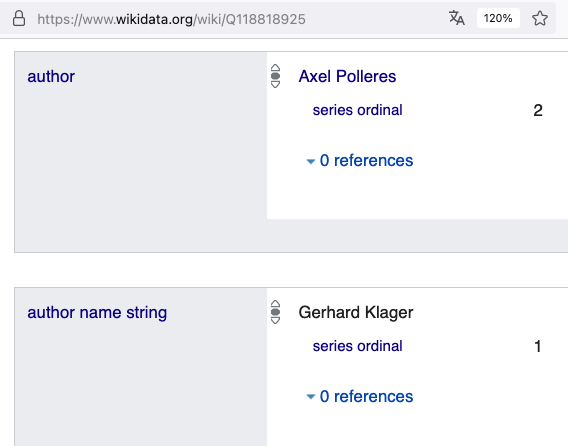
\includegraphics[scale=0.33]{images/author_name_string.png}
    \caption{author name string versus author property}
     \label{fig:author_name_string}
\end{figure}

\footnotelink{http://ptp.bitplan.com}{Proceedings Title Parser}~\cite{Fahl2022} 
has a CEUR-WS parsing mode, which already had the RDFa extractor capability (allowing to cover more recent CEUR-WS volumes using that markup style). Part of this work has been reused and extended to a fully fledged parser in the work we are reporting here.

CERMINE (Content ExtRactor and MINEr)~\cite{Tkaczyk_2015} is a software library and a  \footnotelink{http://cermine.ceon.pl}{web service} for extracting metadata and content from PDF files containing academic publications.
The text content is analysed and a structured XML document containing metadata on, e.g., authors and citations is created\footnote{See CEUR-WS Volume 3352/Paper1.pdf example \url{https://cr.bitplan.com/index.php/CERMINE/Example}}.
The lookup features of CERMINE are limited, e.g., to finding the ISO country code of the country of an institution an author is affiliated with.

GROBID (GeneRation Of BIbliographic Data)~\cite{Lopez_2009} has been gradually extended to be a machine learning library for extracting, parsing and re-structuring raw documents such as PDF into structured XML/TEI encoded documents with a particular focus on technical and scientific publications. 

We have successfully run CERMINE on 68,524 and GROBID on 69,733 CEUR-WS papers so that the results are now a further potential source for disambiguation according to the original challenge tasks 2 and 3.
The corresponding XML files are available via the CEUR-WS single point of truth server see section ~\ref{sec:single_point_of_truth_server}.

\subsection{Scholarly Metadata in Wikidata}

The \footnotelink{https://www.wikidata.org/wiki/Wikidata:WikiCite}{WikiCite} project started in 2014 to work on citation data related to Wikipedia and Wikidata, addressing technical aspects, community building, and the future of open citations. WikiCite is aimed at creating a comprehensive bibliographic database in Wikidata to enhance all Wikimedia projects, with significant progress and community initiatives. As of 2023 the scholarly data in wikipedia is the largest subgraph see \footnotelink{https://www.wikidata.org/wiki/Wikidata:Statistics}{Wikidata Statistics}\cite{AKhatun2021} with 22.6 million scholarly articles providing 31.5\% of the 71.6 million instances as of 2023-12.

The \footnotelink{https://scholia.toolforge.org}{Scholia} project ~\cite{Nielsen2017} utilizes the scholarly data in Wikidata to provide detailed 
profiles for researchers, organizations, journals, publishers, individual scholarly works, and research topics. The Scholia's web portal creates 
on-the-fly scholarly profiles by querying the 
SPARQL-based Wikidata Query Service and 
visualizing the data in various formats. This 
includes lists of publications, author co-occurrence graphs, topic overlays, and more,  significantly enhancing the discoverability and 
analysis of scholarly communication. Scholia's web portal is an open source project hosted on \footnotelink{https://github.com/WDscholia/scholia}{github}. 

\section{CEUR-WS Semantification}\label{sec:Semantification}

\subsection{Overview}\label{sec:sem_overview}
Figure~\ref{fig:ceurmake_workflow} gives an overview of the CEUR-WS Semantification workflow.
The workflow is cyclic -- it starts with what has so far been the single point of truth metadata, i.e., the ones embedded in the HTML/PDF/text of the static publication infrastructure. The Metadata Extraction step parses the input files and creates Metadata Records (which are cached as JSON records and in an SQLite relational database). These form the basis for the Matching/Reconciliation that queries Wikidata, DBLP and GND with the respective SPARQL endpoints. The semantified Metadata Records are now available and may be stored in the format we see fit.  JSON and YAML are candidate formats see table \ref{tab:format_comparisons}. In the next cycle the parsing of existing records is not necessary any more as long as there have been no changes. When new volumes are published, the main page, listing all proceedings volumes, is modified and HTML tables of content and PDF files are added per volume as submitted by the workshop editors. Currently this is done manually via the tradional workflow and semi-automatic via the single point of truth server see section ~\ref{sec:single_point_of_truth_server}.

%\subsection{Steps}
%* Person disambiguation
%** Editor disambiguated with affiliation and homepage
%** id lookup orcid url is given as homepage
%* label lookup + majority vote
%** city and country are resolved to their Qid
%* date range (as text) is parsed from string to proper start and end date
%* NLP
%** ordinal is extracted from proceedings title
%** series title is extracted from proceedings title
%** event is extracted from proceedings title
%** event type (Conference or Workshop)
%* parsing of semi-structured data (html + css classes)
%** acronym
%** event website
%** publication date
%** paper and its authors
%*** Author disambiguation pending
%*** DBLP lookup based on paper title → DBLP author id

\begin{figure}
    \centering
    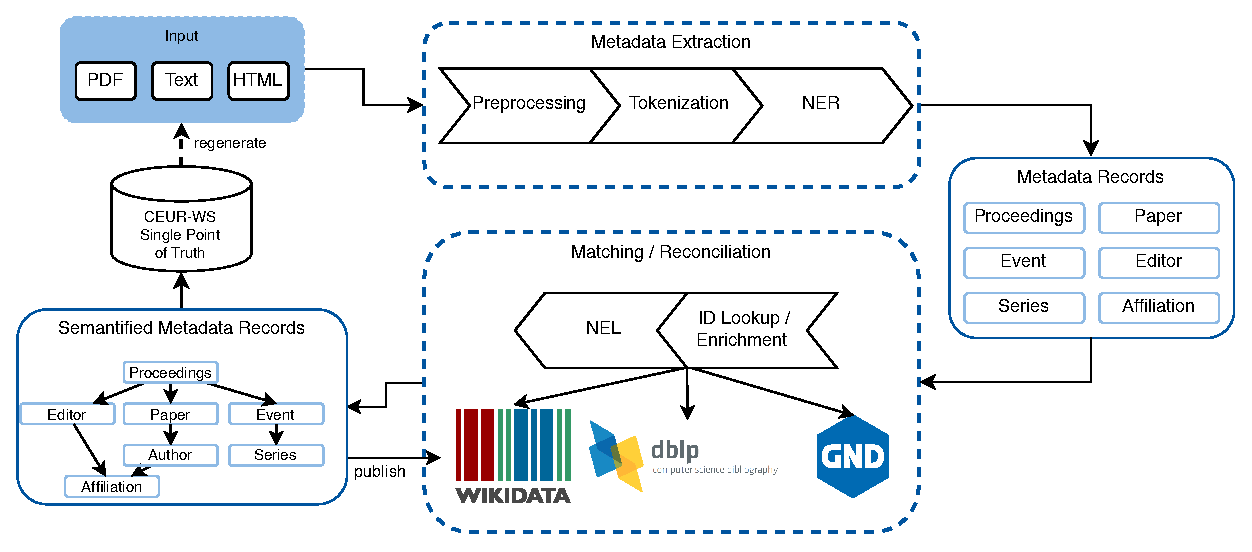
\includegraphics[width=\linewidth]{images/pyceurmake_workflow.eps}
    \caption{Workflow of the CEUR-WS Semantification}
    \label{fig:ceurmake_workflow}
\end{figure}

The steps of the semantification workflow for CEUR-WS as depicted in Figure~\ref{fig:ceurmake_workflow} are explained in the following subsections.

\subsection{Preprocessing}
To extract the relevant markup elements, we created parsers for the index and volume HTML Files as part of the pyCEURMake project. These parsers handle the RDFa-like annotations that have been applied in newer CEUR-WS volumes as well as the special and exotic cases arising from the long tail follow-up problems of the different over 33 styles of HTML structure being used. The BeautifulSoup4 Python library is used for lenient HTML parsing as a basis.

\subsection{Tokenization}

\subsubsection{Disambiguation using Event Signatures}\label{sec:Event_signature}
As outlined in Section~\ref{sec:event_pids}, PIDs would be useful for uniquely identifying scientific events. In the absence of PIDs, it is necessary to use a quasi-identifier~\cite{OECD2008} consisting of a set of metadata elements referred to as \tquote{Event Signature}. There is neither a standardized definition of event signatures nor a recommendation for their use in references and proceedings titles. Retrieving the signature from the volume's textual description is a core step in creating the CEUR-WS knowledge graph. 

As part of~\cite{Franken2022}, the first author of this article has shown
that a typical scientific event \tquote{signature} consists of the following metadata (the example event being \footnotelink{https://www.wikidata.org/wiki/Q48027931}{ISWC 2019} \emph{The Semantic Web – ISWC 2019: 18th International Semantic Web Conference, Auckland, New Zealand, October 26–30, 2019}):
\begin{description}
\item[acronym] a short name for the conference, often consisting of 3 to 8 upper case letters aiming at uniqueness but actually still often being ambiguous.  For instance, ISWC may refer to the \textbf{International Semantic Web Conference} or to the International Symposium on Wearable Computing.
\item[frequency] annual, biennial, triennial -- most events have an \textbf{annual} frequency and this is mostly \textbf{not stated explicitly}.
\item[event reach] target reach of the conference such as \textbf{international}, European, East Asian
\item[event type] such as \textbf{Conference}, Workshop, Symposium  
\item[year] a two or four digit reference to the year in which the event took place -- not to be confused with the year of publication of the proceedings, which might be different (\textbf{2019})
\item[ordinal] often used to enumerate the conference series instances (\textbf{18th})
\item[date] start date and end date or date range of the conference (\textbf{October 26--30})
\item[location] description of the location of the conference often consisting of country, region and city -- sometimes with details about the exact venue. (\textbf{Auckland, New Zealand})
\item[title] the title often contains scope, type and subject of the conference (\textbf{International Semantic Web Conference})
\item[subject] description what the conference is about, often prefixed with ``on'' (\textbf{Semantic Web})
\item[delimiters] a variety of syntactic delimiters such as blanks, comma, colon, brackets are used depending on the citation style.
\end{description}

The event signature needs to be extracted from the CEUR-WS main and volume tables of contents and stored as triples for the target KG. 

The distinction between proceedings, event and event series needs to be made -- therefore the result needs to be split and disambiguated against existing entries in the target KG.

The mapping as outlined in Table~\ref{tab:wikidata_mapping} has been used to map to the \tquote{event} and \tquote{proceedings} entry in Wikidata.  The top rows of the table show the common properties of the proceedings and event item entries, followed by the special properties for events followed by the special properties for proceedings.

The series entry for the Text2KG example has been created and \tquote{colocated} property that has been added as part of this work recently is  filled for this example. The \footnotelink{https://scholia.toolforge.org/event-series/Q116982161}{Text2KG Workshop series Scholia overview} shows the connections.

As an example, we are using the Wikidata entry for the \footnotelink{https://www.wikidata.org/wiki/Q113512465}{Text2KG@ESWC-2022} workshop, whose proceedings have been published as \footnotelink{https://ceur-ws.org/Vol-3184/}{CEUR-WS Volume 3184} with the \href{https://www.wikidata.org/wiki/Q113512180}{Wikidata proceedings item} being shared by another workshop (a special but still frequent case required by the CEUR-WS submission guidelines).

\begin{table}
\caption{Mapping Event Signature Elements to Wikidata}
\label{tab:wikidata_mapping}
%\begin{minipage}{\textwidth}
\begin{tabular}{p{2.5cm}p{3.7cm}p{6cm}}
\toprule
property & PID & example\\
\midrule
acronym     & \wdpTable{short name}{P1813} & Text2KG 2022 \\
title       & \wdpTable{title}{P1476} & 1st International Workshop \newline on Knowledge Graph Generation From Text \\
\midrule
event type  & \wdpTable{instance of}{P13} & Workshop\\
date(start) & \wdpTable{start time}{P580} & May 30\textsuperscript{th}, 2022 → 2022-05-30\\
date(end)   & \wdpTable{end time}{P582} & May 30\textsuperscript{th}, 2022 → 2022-05-30\\
location    & \wdpTable{location}{P276} & Hersonissos → \wdqTable{Chersonesos Irakliou}{Q1018106}\\
country     & \wdpTable{country}{P17}  & Greece → \wdqTable{Greece}{Q41}\\
series      & \wdpTable{part of the series}{P179}  &  International Workshop on Knowledge Graph Generation From Text → \wdqTable{Workshop on Knowledge Graph Generation From Text}{Q116982161}\\
ordinal     & \wdpTable{series ordinal}{P1545} & 1st\\
colocated with & \wdpTable{colocated with}{P11633} & ESWC 2022 → \wdqTable{ESWC 2022}{Q110791806}\\
homepage & \wdpTable{official website}{P856}& \href{https://aiisc.ai/text2kg/}{https://aiisc.ai/text2kg/}\\
\midrule
URN & \wdpTable{URN-NBN}{P4109} & urn:nbn:de:0074-3184-1 \\
publication date & \wdpTable{publication date}{P577} & 2022-08-11 \\
DBLP id & \wdpTable{DBLP publication ID}{P8978} &  conf/esws/2022text2kg \\
k10plus id &\wdpTable{K10plus PPN ID}{P6721} & 1818588285\\
\bottomrule
\end{tabular}
%\end{minipage}
\end{table}

\subsection{Named Entity Recognition and Linking (NER \& NEL)}
The Named Entity Recognition (NER) and Named Entity Linking (NEL) tasks for the CEUR-WS Semantification are based on the textual input from the HTML markup that needs parsing into tokens that represent entities, and then matching the textual content of the tokens against Wikidata entries that might need disambiguation. 

The semi-structured HTML markup is simpler to handle than natural language processing of plain text since the parsing of the different entity types can be guided by structural hints such as expecting a title in an \texttt{h1} HTML tag context and therefore increases the accuracy of the matching process~\cite{COCHINWALA20011}.
Items to disambiguate are derived from the event signature as outlined in section \ref{sec:Event_signature}: Volumes, Papers, Editors, Authors, Locations (Country/Region/City), Dates, Ordinals, Acronym, Homepage.

For the phase of the project we are reporting, the mass creation of Proceedings and Event entries was in the focus. The Paper, Editor and Author disambiguation and Event series completion has been prepared and example results are available to show that the elements are available and may be systematically created and queried.
%as we intend to do  mass-creation of Wikidata items after the green light from our legal department which is due after the publication of this work. 
%data reconciliation~\cite{MoEl1996}~\cite{KiCR2023}
\subsubsection{Location NER and NEL}
The location of an event is described in the table of contents in \textit{span} elements usually classified as \textit{CEURLOCTIME}.
Their value contains semi-structured information about the event's location and date range, e.g., \tquote{Hersonissos, Greece, May 30\textsuperscript{th}, 2022}.
Besides the varying formats of the location and date definition, the location information can be fairly easy separated from the date.
This leaves a string that should contain information about the city and country.
There exist cases where also the region or venue is named, and since more and more conferences have moved to virtual meetings since 2020, the location string could also contain indications for that.
Since location strings can be identified on extraction, Named Entity Recognition (NER) and Named Entity Linking (NEL) are done in one step to get Wikidata QIDs of the mentioned locations.
For the NEL we used geograpy3, a Python library that has a database with the labels of countries, regions and cities in multiple languages linking to the corresponding Wikidata QID.
The response of this label lookup is a list of possible locations of the aforementioned categories.
The list is sorted by the category order city, region, country where the cities are also ordered by population.
To this list, we once more apply a ranking, since we know that in most cases the country is named within the string, so we can select the city in the given country context.
For the given example the result would then be \tquote{Hersonissos, Greece} → \wdq{Chersonesos Irakliou}{Q1018106} (\wdq{Greece}{Q41}).

\subsubsection{Editors and Authors}
The author and editor name disambiguation is one of the main challenges for libraries and indexers~\cite{Subramanian_2021}.
Due to the common occurrence of duplicate names, abbreviations of first names, typos and encoding errors disambiguation is an expensive and error-prone task if high accuracy is aimed for.

In CEUR-WS, the editor information is given in an HTML element containing the editor signature, usually given name and family name with a numeric reference to the affiliations, as shown in Listing~\ref{listing:editor_span}.
\begin{listing}
\caption{CEUR-WS volume page HTML markup excerpt of editor definition}
\label{listing:editor_span}
\begin{minted}{html}
<b> TEXT2KG edited by </b>
</p><h3>
   <span class="CEURVOLEDITOR">Sanju Tiwari</span> ... 1
   <span class="CEURVOLEDITOR">Nandana Mihindukulasooriya</span> ... 2
   <span class="CEURVOLEDITOR">Francesco Osborne</span> ... 3 4
   <span class="CEURVOLEDITOR">Dimitris Kontokostas</span> ... 5
   <span class="CEURVOLEDITOR">Jennifer D’Souza</span> ... 6
   <span class="CEURVOLEDITOR">Mayank Kejriwal</span> ... 7
</h3>
\end{minted}

\end{listing}
For newer publications, ORCIDs of Authors and Editors might be directly available from the PDF input.
For older volumes, only the plain name, affiliation and no identifier is provided that could simplify the disambiguation.
Fortunately, 78\% of the volumes are indexed at DBLP – less than 800 early volumes are missing.
DBLP provides high quality disambiguated data about the proceeding editors and paper authors also accomplished through manual curation~\cite{Kim_2018}.
Therefore, extracting the editors and resolving each name to an identifier by looking up the DBLP id seems to be the best option.
The same strategy as used for the editors also applies to the authors but here the affiliation needs to be extracted from the paper PDF in the future.

\subsection{ID Lookup/Enrichment - DBLP, k10plus Volume matching and linking}
DBLP and k10plus records may be trivially matched by the unique identifier volume number of a proceeding combined with the URN of the CEUR-WS proceedings series.

We are using the QLever DBLP SPARQL endpoint mentioned in Section~\ref{sec:Introduction} to match CEUR-WS volumes against DBLP entries by volume number.

For the k10plus matching we use the catmandu library, which allows to query the PICA~\cite{Costers1997} (a library cataloging format used predominantly in German-speaking countries) based k10plus database for URN matches; for details, see the \footnotelink{https://w.wiki/6Qm5}{PPN/Volume/WikidataItem matching SPARQL Query}. 

Based on the resolved IDs from the ID lookup and NEL, we can now enrich our data by querying additional or missing data.
For example, in \footnotelink{https://ceur-ws.org/Vol-3356/}{Volume 3356}, only \tquote{Tokyo} is defined as location; linking the string to \wdq{Tokyo}{Q1490} then enables querying for the missing country information.
Similar enrichments are done for editors and authors to complete the records.

\subsection{Decision to use Wikidata as a target}\label{sec:wikidata_decision}
Wikidata~\cite{Vrandecic2014} is a knowledge graph based on an RDF triple store that has been successfully used to gather and link metadata of scholarly communication artifacts~\cite{Nielsen2017}. 

In 2022, we decided to directly target Wikidata instead of trying to set up our own RDF/SPARQL endpoint, as outlined in Section~\ref{sec:sempub_challenge}. 
Wikidata is well suited to to handle the challenges listed in Section~\ref{sec:fair_challenges} as referenced below by priority:
\begin{itemize}
    \item \textbf{Unique Identifiers (F1)}: by assigning Q-Identifiers, such as Q5 for human.
    \item \textbf{Rich, Identifiable Metadata (F2, F3)}: by being originally based on Wikipedia entries from multiple countries and using a very large community and bots to add current items.
    \item \textbf{Searchable Data (F4)}: by providing a robust Wikidata Query Service .
    \item \textbf{Curation and Accessibility (A1, A2, R1.2)}: by enabling community edits and offering multiple language support.
    \item \textbf{Complex Queries Support (A1, I1, I2, I3)}: by facilitating sophisticated querying through a SPARQL endpoint which may be federated with other Linked Open Data endpoints.
    \item \textbf{Ontology Reuse (I1, I2)}: by integrating and linking to external ontologies and databases and providing its own robust ontology curation process.
    \item \textbf{Stability and Trust (R1.3)}: by ensuring stability and trust through Wikimedia Foundation governance and having mirrored data in for profit (e.g. google) and non profit organizations\footnote{e.g. RWTH Aachen i5 runs multiple copies of Wikidata!}.
    \item \textbf{Open Source, Non-Profit (R1.1)}: by promoting an open-source, non-profit model with Wikimedia Foundation and community contributions.
\end{itemize}





\subsection{Workshop colocated with conference}
Most CEUR-WS Volumes are proceedings of workshops, whose majority is colocated with a conference. For this \tquote{colocation} relation there was no specific property in Wikidata when we started the semantification. Kolchin~\cite{Kolchin2015} had already pointed out that \tquote{BIBO doesn't have an `event is part of bigger event' semantics} in 2015, so the need was long known.
We initiated the creation of \wdp{P11633}{colocated with} by a \footnotelink{https://www.wikidata.org/wiki/Wikidata:Property\_proposal/colocated\_with}{property proposal} according to the \footnotelink{https://www.wikidata.org/wiki/Wikidata:Property\_proposal}{Wikidata's property proposal process} which states \tquote{When after some time there are some supporters, but no or very few opponents, the property is created by a property creator or an administrator.}

\footnote{One further criterion was that at least three examples need to be supplied. Unfortunately we did present a few dozen examples but not in the format expected which held up the process by a few months}.

After that, there was a lively and productive discussion that lead to the clarification that the property is asymmetric. The property was considered as highly relevant and well defined. After almost a year of preparation and discussion the Property is now available and shall be used in the future.

\section{SemPubFlow}\label{sec:SemPubFlow}

\subsection{Overview}
SemPubFlow represents a transformative approach in the lifecycle of 
scientific events as outlined in Table~\ref{tab:ScientificEventLifecycle}, advocating for early curation and integration of  publicly available machine-readable metadata separating the concerns of content and visualization.

Traditionally the created artifacts are mostly intended for human consumption and therefore optimized in this respect. Table~\ref{tab:format_comparisons} shows the computer readability challenges of some of the most common formats which often need sophisticated natural language processing capabilities to be performed. A limiting factor is the lack of standardization and separation of concerns. With the advent of LLMs the options for processing these diverse sources of metadata are vastly improving---making it feasible to get computer readable results as early as possible. 

\begin{table}
\centering
\begin{tabular}{|p{2.5cm}|p{9.5cm}|}
\hline
\textbf{Format} & \textbf{Description} \\
\hline
Plain text & Requires natural language processing (NLP) for metadata extraction due to its unstructured nature.\\
\hline
HTML & Readability varies with the structural and semantic rigor in the document. Microformats and RDFa are sometimes available. \\
\hline
PDF & Primarily being a collection of individual glyphs to be positioned and formatted, pose challenges in text reconstruction and structure analysis. \\
\hline
BibTeX & Structured nature makes it highly suitable for computer readability and metadata extraction in scholarly communications. \\
\hline
XML/JSON/YAML & Markup languages that balance human and machine readability with varying degrees of structure strictness. \\
\hline
RDF & A standard model for data interchange, facilitating data merging and schema evolution support across diverse schemas. \\
\hline
Multimedia (Videos, Pictures)& Visual media often require sophisticated processing such as  OCR for text extraction a for content extraction. \\
\hline
Other (PPT, Word, SVG, etc.) & Vary in readability; structure and semantics can usually be accessed via specific APIs or tools\\
\hline
\end{tabular}
\caption{Computer Readability of various formats used for scholarly artifacts}
\label{tab:format_comparisons}
\end{table}


%\href{https://tw.rpi.edu/project/rdesc}{RDESC} (Resource Discovery for Extreme Scale Collaboration) \cite{Purohit_2016} was a project 

\subsection{Traditional CEUR-WS Submit Workflow}
CEUR-WS describe their publishing procedure in a detailed submission guide~\cite{CEURHowtoSubmit}. Figure~\ref{fig:howtoworkflow} provides an overview of this workflow as an UML activity diagram.
Even use of \tquote{PUT} in the workflow description indicates that the workflow has been in place since 1995 mostly unchanged with the idea of collecting and uploading PDF-Files and creating per Volume html pages with a single monolithic index.html to list them all.

\begin{figure}
    \centering
    %\includesvg[width=\linewidth]{images/HowToWorkflow.svg}
     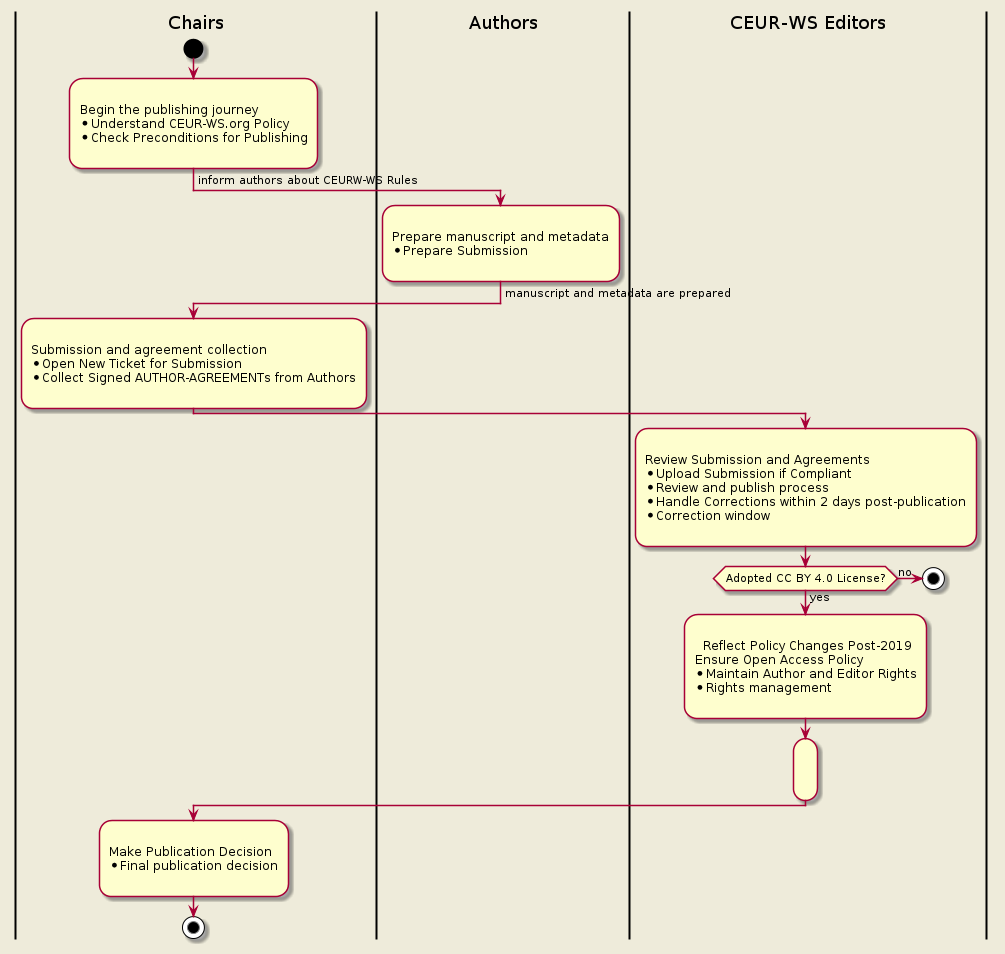
\includegraphics[width=\linewidth]{images/HowToWorkflow.png}
    \caption{CEUR-WS HOWTOSUBMIT workflow}
     \label{fig:howtoworkflow}
\end{figure}
%Even the name "PUT" indicates that the workflow has been in place since 1995 mostly unchanged with the idea of collecting and uploading PDF-Files and creating per Volume html pages with a single monolithic index.html to list them all.

\subsection{Metadata first semantic publishing}
\label{sec:metadata_first}

A key goal of metadata first semantic publishing is the early use (and enforcement of this use) of persistent identifiers. Without such identifiers it is notoriously difficult to disambiguate the core entities involved in scholarly publishing. 

The following PIDs are already often in use but the enforcement of their use is lacking in CEUR-WS. 
\begin{itemize}
    \item \textbf{ORCID (Open Researcher and Contributor ID):} Identifier for individual researchers.
    \item \textbf{ROR (Research Organization Registry):} Identifier for research organization.
    \item \textbf{Wikidata-ID:} A general identifier for entities in the Wikidata database, often making further identifiers available for reference.
    \item \textbf{DOI (Digital Object Identifier):} A general identifier for objects accessible on the internet – often used for scholarly papers.
\end{itemize}


We propose to make the use of PIDs mandatory for publishing in CEUR-WS. Given the existing index entries of CEUR-WS Volumes in DBLP and the German national library, the DBLP and GND identifiers are also candidates. For ORCIDs, RORs, DOIs there is active action required by the stakeholders to obtain these, and, in the case of DOIs, there is cost involved. Using Wikidata as the general PID Infrastructure is much more feasible since it offers a freely accessible, community-driven platform that PIDs for a wide range of entities. This approach aligns with the open and collaborative nature of scholarly communications and meets the requirements for easy integration, broad adoption, and maintenance. Using Wikidata Q-Identifiers as PIDs relies on the long term availability of Wikidata which is quite likely giving the support by a strong community and big commercial players such as google. 

The Wikidata PID usage proposal calls for looking up or creating Wikidata entries for all relevant core entities as early as possible and linking these entries to the standard PIDs where applicable. 

In the workflow the existing entries will later be reusable for computer assisted lookups as part of the SemPubFlow tool see section \ref{sec:sempubflow_tool} and Scholia. 

Figure~\ref{fig:metadata_first_workflow} shows the proposed future 
workflow. Publication via CEUR-WS would ideally involve assigning the 
Volume number and transferring the metadata-rich candidate 
snapshot to the Single Point of Truth. This process ensures the completeness and quality of the metadata allowing for the generation of  traditional HTML pages and the official stamping as a CEUR-WS  proceeding.

\begin{figure}[ht]
    \centering
    %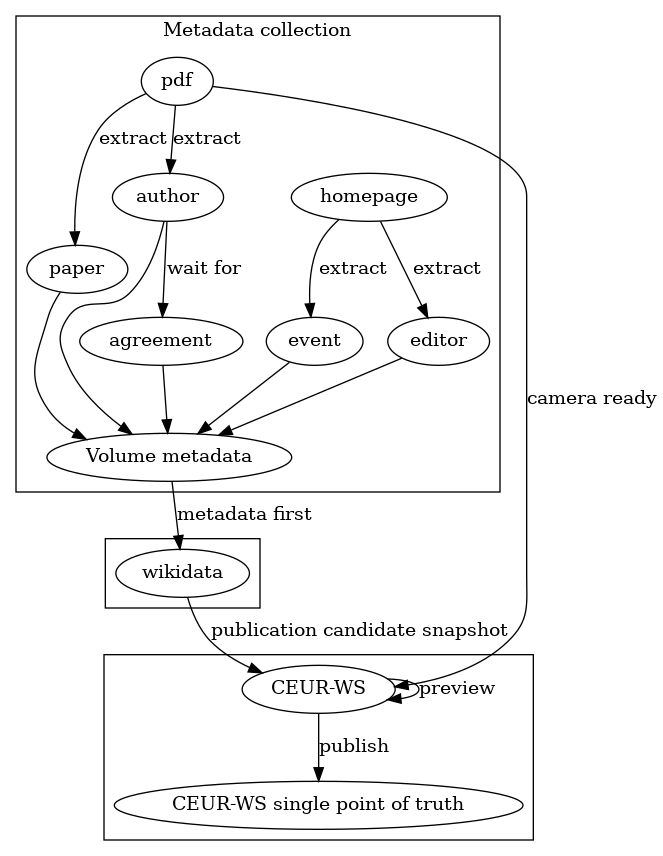
\includegraphics[scale=0.4]{images/MetadataFirstWorkflow.png}
    \includesvg[scale=0.5]{images/MetadataFirstWorkflow.svg}
    \caption{Metadata First Scholarly Publishing Workflow Overview}
    \label{fig:metadata_first_workflow}
\end{figure}
\subsection{Iterative introduction}
The software engineering challenge in introducing the SemPubFlow workflow is to find a sweet spot between effort and benefit~\cite{Pohl2015-vj}. Given the long-tail distribution of issues of ever more corner and exotic cases that have shown up in the analysis of the existing data and workflow there is potentially a huge list of \tquote{small} problems that would require an inadequately high amount of effort to be solved systematically. The \tquote{sweet spot} is in solving only the most relevant problems and not fixing some of the exotic details at all or doing it manually. Therefore we will avoid a \tquote{big bang} introduction, which would replace  the old workflow with the new SemPubFlow in one single big (and therefore very risky) step.
Instead we propose to do smaller changes gradually. As a first step, the main index.html shall be split by years (with a link to the old legacy complete list). Then, the per-year list may be partly created using the new SemPubFlow approach. This will be continued iteratively, going from the current year back to a point where it seems not reasonable any more to spent further effort. 

\subsection{Legal aspects of Publishing Personal Data of Scholars}
\label{sec:legal}
The proposed workflow calls for publishing personal data of authors and editors early in the life cycle of an event.

This is perfectly legal under at least one of the following conditions:\footnote{Disclaimer: this is just a summary in layman's terms of legal analysis that was done as part of the CEUR-WS semantification project}

\begin{enumerate}
    \item \textbf{Consent:} Explicit consent from individuals for their data to be published – e.g., by signing an authors agreement.
    \item \textbf{Legitimate Interests:} Publication serves legitimate interests that outweighs the individual's rights and freedoms. E.g., when the scholar is a person of public interest.
    \item \textbf{Public Data:} Data has already been made public by the scholar.
    \item \textbf{Scientific Research:} Processing is necessary for scientific research purposes as per Article 89 of the GDPR.
    \item \textbf{Contractual Necessity:} Necessary for the performance of a contract with the scholar – e.g., publishing a paper in workshop proceedings and making the metadata available for indexing by Wikidata, dblp, libraries and other interested parties.
    \item \textbf{Legal Obligation:} Necessary for compliance with a legal obligation. This would, e.g., be the case if the publication was done via a traditional print outlet and thus, by German law, a copy of the proceedings has to be made available to the German National Library. On indexing, the personal data records of authors will be created as part of the German National Library's legal commitment.
    \item \textbf{Vital Interests:} Necessary to protect the vital interests of the scholar or another person. This category is more relevant to medical or emergency situations and rather unlikely to be applicable for the scholarly publication use case.
    \item \textbf{Public Interest:} Necessary for performing a task carried out in the public interest or in the exercise of official authority. E.g., when an investigation by public  authorities is underway. 
\end{enumerate}

Consent, Public Data, and Contractual Necessity are crucial for scholarly publishing. Considering the analogy with Legal Obligations applying to print outlets, we expect it to be feasible to convince scholars that publishing their necessary personal data is reasonable in digital contexts.

\section{Implementation and Demos}
\label{sec:implementations_and_demos}

\subsection{Open Source}
The CEUR-WS semantification projects are open sourced via the repositories of the  
\footnotelink{https://github.com/ceurws}{github ceurws organization}. 


A \footnotelink{http://ceur-ws.bitplan.com}{prototype for the presentation} of the CEUR-WS Semantification results has been created using Semantic MediaWiki~\cite{Kroetzsch2011} (SMW), which is using the same MediaWiki open source engine as Wikipedia. SMW has extensions for markup that is transforms subject-predicate-object statements to triples, which leads to a \tquote{Semantification} of the Wiki by making the triples available for query.
Like most SMW installations we are using the standard SQL based triplestore and ask queries and not RDF/SPARQL \cite{Fahl2020}. 

A GitHub project for the single-point-of-truth metadata handling and conversion to different representations has been started at \footnotelink{https://github.com/ceurws/ceur-spt}{ceurws/ceur-spt}. 

Further background research material is supplied via the Semantic MediaWikis for \footnotelink{https://cr.bitplan.com/index.php/Category:Text2KG}{Wolfgang Fahl's PhD} (public) and the \footnotelink{http://rq.bitplan.com}{ConfIDent requirements wiki} (access on request). 

\subsection{CEUR-WS Volume Browser}
\begin{figure}[ht]
    \centering
    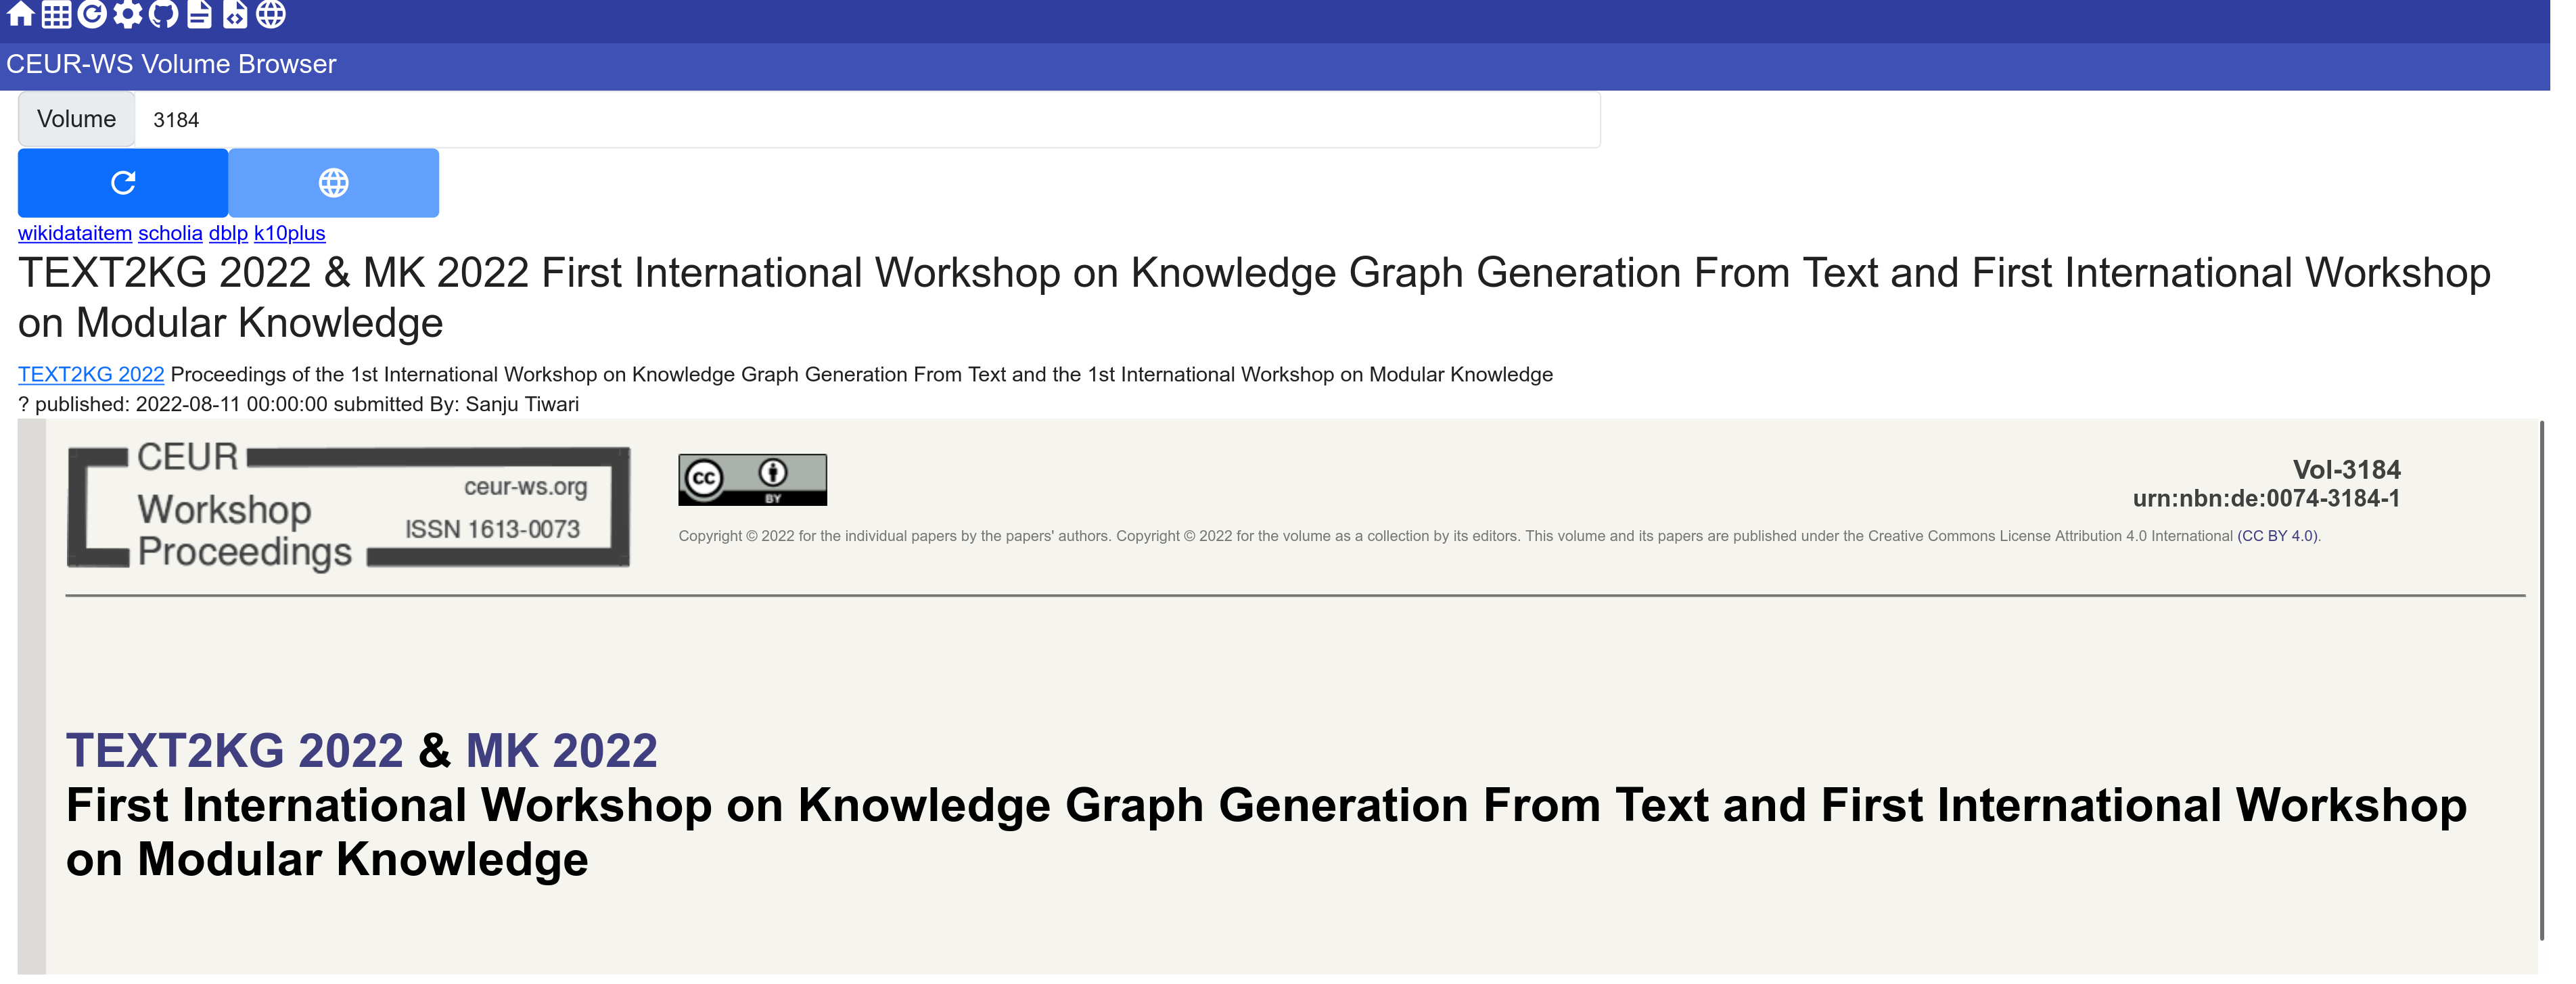
\includegraphics[width=\linewidth]{images/cvb_screenshot.png}
    \caption{Screenshot of the CEUR-WS Volume Browser}
    \label{fig:cvb_screenshot}
\end{figure}
Figure~\ref{fig:cvb_screenshot} shows a screenshot of the CEUR-WS Volume Browser, which we created as a means to support semantification tasks such as transferring metadata of recently added volumes to Wikidata as well as showing the available index entries for volumes that have been published for a few weeks/months already. The example shown is for \footnotelink{https://ceur-ws.org/Vol-3262/}{CEUR-WS Volume 3262 Wikidata Workshop 2022}.  

\begin{figure}[ht]
    \centering
    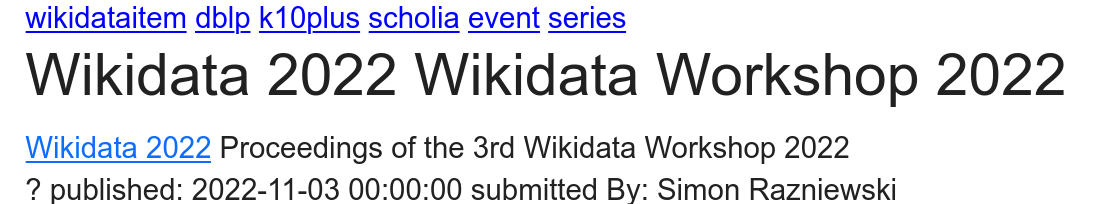
\includegraphics[width=\linewidth]{images/cvb_volume_browser_enlarged.png}
    \caption{CEUR-WS Volume Browser enlarged details with links to external KGs}
    \label{fig:cvb_details}
\end{figure}
Figure~\ref{fig:cvb_details} shows an enlarged section of the screenshot where the links between the proceedings volumes and the external knowlede graphs are presented. In the example, these are \footnotelink{http://www.wikidata.org/entity/Q115053286}{wikidataitem}, \footnotelink{https://dblp.org/db/conf/semweb/wikidata2022}{dblp}, \footnotelink{https://opac.k10plus.de/DB=2.299/PPNSET?PPN=1830580760}{k10plus}, and the Scholia links to the proceedings, event and \footnotelink{https://scholia.toolforge.org/event-series/Q106429025}{event series} (which has links to the event and proceedings). 


\subsection{CEUR-WS Single Point of Truth Server}
\label{sec:single_point_of_truth_server}
The Single Point of Truth Server serves as a prototype and proof of concept for the CEUR-WS semantification. Instead of static HTML, all content displayed by this server is generated from the semantified metadata. The separation of concern of metadata and presentation is implemented here. 

The server software is available open source at \footnotelink{https://github.com/ceurws/ceur-spt}{github}. It runs on  uvicorn ASGI server and FastAPI web framework and has only a limited list of dependencies to stable Python libraries for long term maintainability. 

Key features are HTTP content negotiation for human (HTML) and computer (JSON,YAML,XML, ...) consumption and a documented RESTFul API. 

The demo of the server is available at the 
\href{http://ceurspt.wikidata.dbis.rwth-aachen.de/index.html}{RWTH Aachen i5 chair}. 

Using FastAPI version 0.1.0 with \footnotelink{https://swagger.io/specification/}{Swagger OAS3} compatibility, a comprehensive set of endpoints is offered. There are endpoints which are compatible with the traditional static for index and volume HTML tables of contents, as well as paper PDFs that deliver HTML content. In addition various other computer readable representations are available. 

Notably, each paper is accessible via a dedicated endpoint,
a feature absent in the traditional static CEUR-WS implementation.
Links to corresponding volumes and author indices (dblp, GND,
and Wikidata) are provided, while granting direct access to Scholia
profiles based on the Wikidata items.

The paper endpoint enables retrieval of both the PDF and its
plain text. It integrates the CERMINE and GROBID results for
advanced XML analysis. The metadata can be exported as
QuickStatements for Wikidata, wikibase-cli, Semantic MediaWiki
Markup, or in standard formats such as JSON or YAML,
facilitating interoperability and analysis for different use cases.
Individual entity imports and amendments for different target
platforms are thus possible. This is a step towards the scholarly
CMS concept presented in section \ref{sec:future_work}.

Figure~\ref{fig:ceur-spt-screenshot} shows an example paper from the second TEXT2KG@ESWC2023 workshop. 
\begin{figure}
    \centering
    %\includesvg[width=\linewidth]{images/HowToWorkflow.svg}
     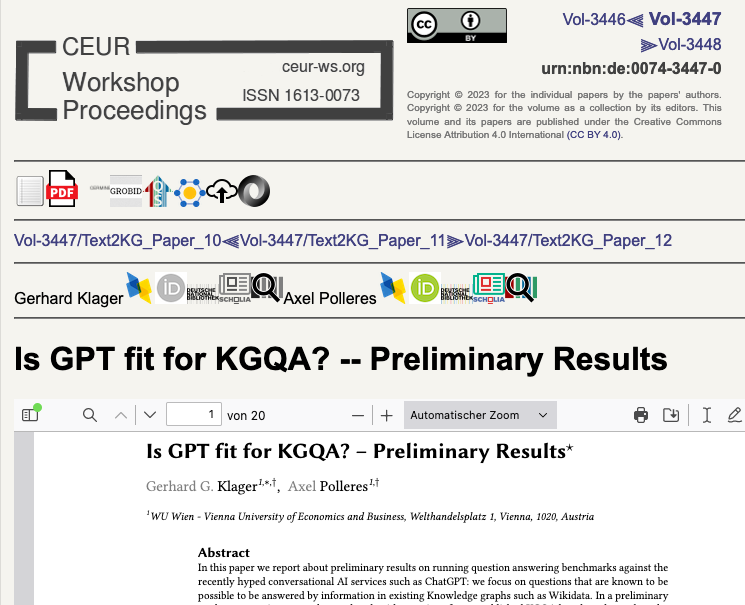
\includegraphics[width=\linewidth]{images/ceur-spt-screenshot2023-12-29.png}
    \caption{Paper landing page of CEUR-WS Single Point of Truth server}
     \label{fig:ceur-spt-screenshot}
\end{figure}

When scholars change their name over time they are often inclined to ask to have their name changed in the original publications. While this is mostly not feasible the paper endpoint approach with an author bar allows to display the new name. 




\subsection{Single Point of Truth against Wikidata validation}
A major concern of the CEUR-WS editors and other stakeholders is the trustworthiness of the Wikidata entries. These entries are mostly created by the CEUR-WS Wikidata bot but also by other tools such as Scholia and individual Wikidata curators. 
Therefore, it is necessary to regularly check that the single point of truth data is consistent with the Wikidata entries. This is especially important for the identifiers being used. The pyLodStorage synchronization tool (see section ~\ref{sec:ack}) checks the consistency. Table~\ref{tab:URNSync} shows an example result for the URN-NBN persistent identifier. In 580 cases the URN identifier is set in Wikidata (since the URNs can be calculated from the volume number as explained below) but not available from the volume pages via a microformat annotation such as
\begin{minted}{html}
<span class="CEURVOLNR">Vol-3601</span>
\end{minted}
as was the case for very early volumes.

In 17 cases, there was a mismatch originating from mistakes in the manual execution of the traditional workflow. These cases have been checked manually and could be partly fixed via the wikibase-cli command line tool with generated fixing commands such as: 
\begin{minted}{bash}
$ wd add-claim Q116525021 P4109 "urn:nbn:de:0074-3249-2"
\end{minted}

However, some of the URN entries where wrong in the input Volume HTML files see Table~\ref{tab:dnbtool}. Finding these problems was notoriously difficult since the documentation of DNB URN-NBN check digit generation is obscure and the website tool for generating the check digits does not have an API (see \footnotelink{https://github.com/WolfgangFahl/pyCEURmake/issues/88}{CEUR-Make issue 88} for the details) \footnote{different versions of the tool in Javascript, PHP and python needed to be compared due to the C-puzzle book style handling of pos++ in the code.}.
\begin{table}
\centering
\begin{tabular}{|l|l|}
\hline
\textbf{Volume}                      & \textbf{URN}              \\\hline
\href{https://ceur-ws.org}{Vol-2018} & urn:nbn:de:0074-2018-6    \\\hline
\href{https://ceur-ws.org}{Vol-2210} & urn:nbn:de:0074-2212-3    \\\hline
\href{https://ceur-ws.org}{Vol-2479} & urn:nbn:de:0074-2479-C    \\\hline
\href{https://ceur-ws.org}{Vol-2743} & urn:nbn:de:0074-2743-1    \\\hline
\href{https://ceur-ws.org}{Vol-2843} & urn:nbn:de:074-Vol-2843-4 \\\hline
\href{https://ceur-ws.org}{Vol-3419} & urn:nbn:de:0074-3419-9    \\\hline
\href{https://ceur-ws.org}{Vol-3466} & urn:nbn:de:0074-XXX-1     \\\hline
\end{tabular}
\caption{URN checksum Check}
\label{tab:dnbtool}
\end{table}
\begin{table}
\caption{URN-NBN Synchronization}
\label{tab:URNSync}
\begin{tabular}{rclrr}
\hline
    left &  $\leftrightarrow$  & right    &    \# &      \% \\
\hline
 CEUR-WS &  $\leftarrow$  & Wikidata &  580 & 16.10\% \\
 CEUR-WS &  $\leftrightarrow$  & Wikidata & 3006 & 83.43\% \\
 CEUR-WS &  $\rightarrow$  & Wikidata &   17 &  0.47\% \\
\hline
\end{tabular}
\end{table}

\subsection{Metadata Query capability}
Having the CEUR-WS metadata available in Wikidata allows for standard SPARQL queries, e.g., using the Wikidata Query Service, to be applied to analyze it. Figure~\ref{fig:cvb_screenshot} shows a map of the distribution of event locations created with such a query. 
\begin{figure}
    \centering
    %\includegraphics[width=\linewidth]{ceur-ws_events_map.png}
    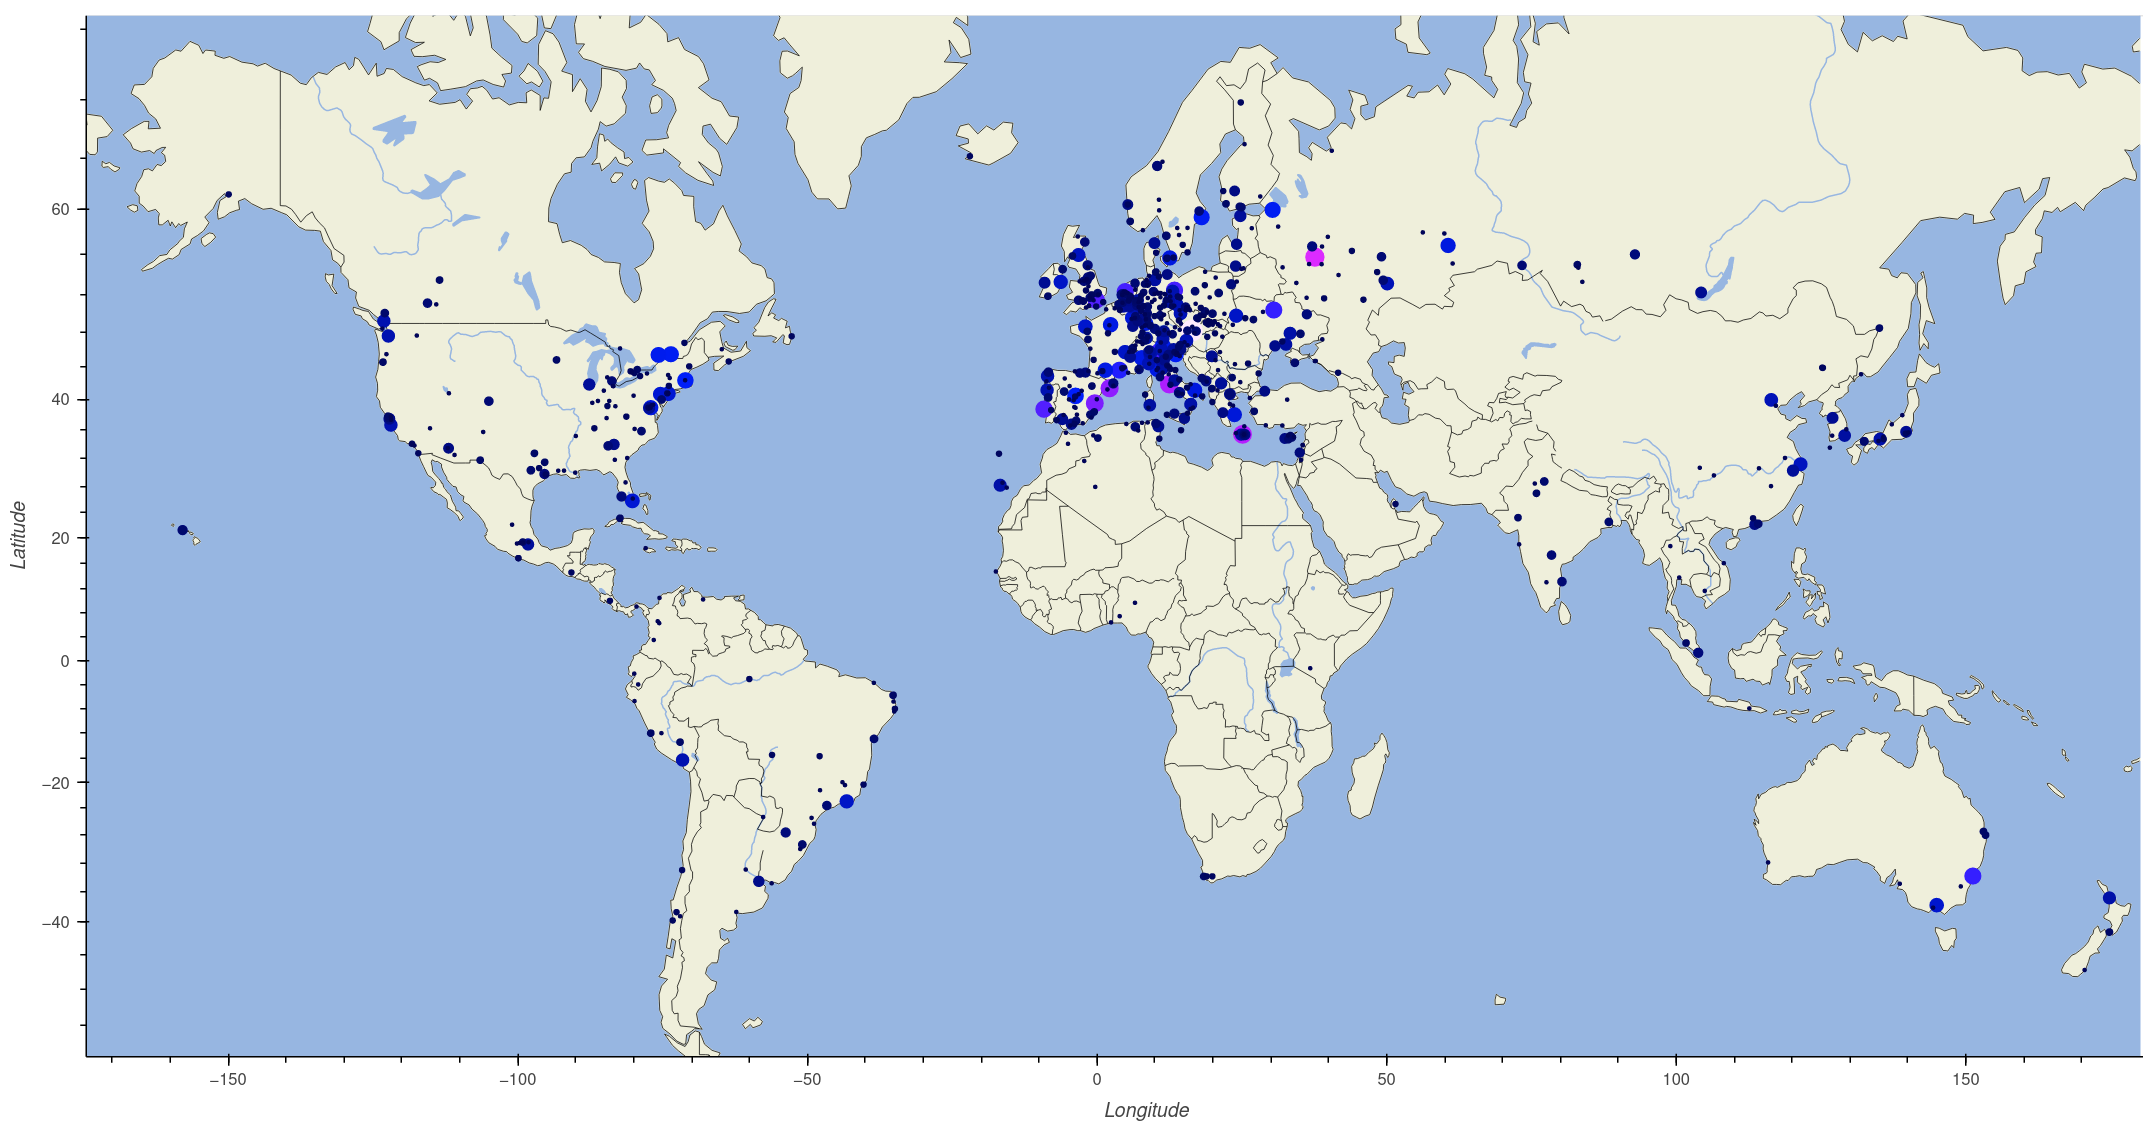
\includegraphics[width=0.8\linewidth]{images/ceurws_event_locations_alternative.png}
    \caption{Locations of all CEUR-WS proceedings events (\href{https://cr.bitplan.com/index.php/Q0.10}{Query 0.10})}
    \label{fig:event_map}
\end{figure}
The relevance of the original set of 20 queries for Task~1 of the Semantic Publishing Challenge, which were set as a benchmark in 2014 for different stakeholders, was subjectively rated by us, resulting in \footnotelink{https://cr.bitplan.com/index.php/List\_of\_Queries}{a list sorting the queries by priority}. The most relevant queries and the 5 queries Q1.5, Q1.12, Q1.13, Q1.16 and Q1.17 that rely on the main index have been implemented as \footnotelink{https://cr.bitplan.com/index.php/Semantic\_Publishing\_Challenge\_Queries}{SPARQL queries} that are compatible with the Wikidata Query Service endpoint to prove that our approach covers the intentions of the original challenge.  Our result supplies even more capabilities given the option to run federated SPARQL queries over the connected Wikidata, DBLP and k10plus knowledge graphs. The use of Wikidata IDs as persistent identifiers is a core success factor here.

\subsection{Evaluation by Further Quality Metrics}
Making the CEUR-WS Volume metadata available on Wikidata has improved the indexing \textbf{coverage} to 100\% of all valid Volumes compared to 69\% for k10plus and  76\% for dblp.

%Check against dblp/k10plus (wikicfp) ...

The \textbf{timeliness} of the CEUR-WS metadata in Wikidata is much higher than for DBLP or k10plus. For DBLP it takes a few days to weeks, for k10plus it may take weeks to months before the metadata shows up. The Wikidata update may be done immediately when publishing with no delay - with SemPubFlow the data will be available as early as the event organizers see fit. With the separation of event and proceedings entries it is now possible to show future events for which there are no proceedings available yet as soon as the events have been announced, and later link the detailed proceedings metadata to the event record.

\section{Conclusion}\label{sec:Conclusion}
We have presented the first steps of CEUR-WS Semantification that result in the metadata of CEUR-WS Volumes being available in Wikidata. The linking of the relevant entities for workshops, the conferences these workshops might be colocated with, the event series that these workshops and events might form, as well as the linking to editor, author and paper entries and the affiliated institutions has been prototyped. 

The cross-linking with DBLP and k10plus has been performed and may now be continuously applied in the future.

Given that all four involved meta data sources -- CEUR-WS, Wikidata, DBLP and k10plus -- involve a lot of manual curation, data quality errors deriving from human errors still have to be mitigated with the goal to achieve a lower error rate than would be possible with manual efforts alone.


\subsection{Future Work}
\label{sec:future_work}
\begin{figure}
    \centering
    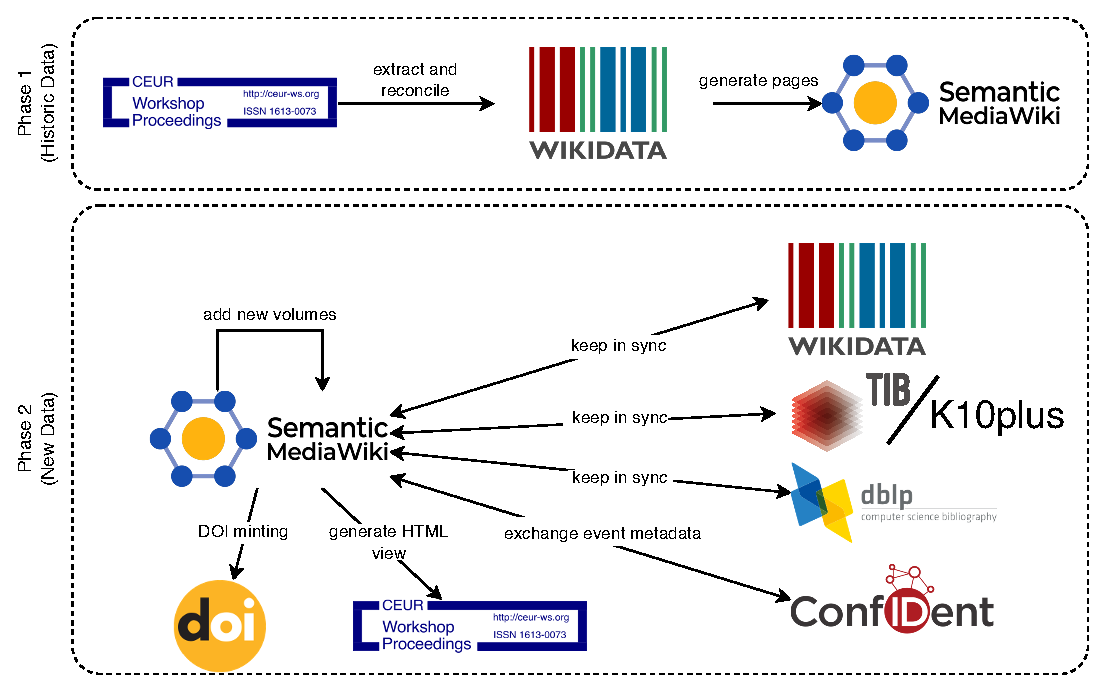
\includegraphics[width=0.8\linewidth]{images/CEUR-WS-SemantificationOverview.eps}
    \caption{CEUR-WS Semantification}
     \label{fig:sem_overview}
\end{figure}

Figure~\ref{fig:sem_overview} shows an overview of a possible new approach to publishing via CEUR-WS. The core idea is to separate the concerns of displaying content (such as static HTML/Semantic MediaWiki) from the storage of metadata in a knowledge graph, e.g., Wikidata. 

The new publishing workflow shall be based on single-point-of-truth metadata that is kept in a computer readable format such as JSON and generate the HTML presentation from this metadata. 

CEUR-WS papers do not have DOIs assigned to them during the publishing process. Assigning DOIs to papers is a feature much asked for by workshop organizers these days, which CEUR-WS did not supply in the past. The new approach/architecture would simplify the DOI minting, since the necessary metadata is a subset of the metadata we intend to provide anyway.

The first phase shows the current state of the workflow in the prototype phase, which we report on in this paper, while the second phase is the goal of the \tquote{Semantification} project hat has been officially started in February 2023 by the CEUR-WS Editors' team. 

Mass creation, editing and disambiguation of relevant scholar entries in Wikidata has to be performed to make these entries available for lookup and reference by the SemPubFlow tool. We intend to build on the Scholia experience with this type of task. 

The LLM approach already proven successful for volume homepages needs to also be applied for the much larger data sets of author homepages. An interesting research question is how well the pre processing of PDF files with CERMINE and GROBID is helpful in getting extraction and disambiguation results for paper metadata and how that might influence the efficiency, cost and accuracy. 

Given the promising aspects of SemPubFlow, community feedback 
is essential for its iterative development to better meet 
the evolving needs of the academic ecosystem. Allowing the 
integration with other publishing outlets besides CEUR-WS 
will be a key success factor. Future enhancements will have to focus 
on increasing the automation and accuracy of metadata 
extraction and management, while ensuring the tools developed 
are accessible, user-friendly and well integrated with the publishing workflow.

In promoting metadata-first publishing, a public infrastructure like 
Wikidata could be used to dynamically generate artifacts, including 
homepages, CfP webpages, emails, and marketing materials, thus 
eliminating tedious manual tasks and forming a generic scholary content management system. This approach requires addressing 
the balance between standardization and individualization, ensuring 
that while a common framework is maintained for FAIRness and efficiency, 
the unique aspects of individual publications are not lost. Key to this 
is the separation of concerns: maintaining distinct layers for metadata 
storage, content generation, and presentation, allowing each to evolve 
independently while cohesively contributing to the scholarly publishing 
ecosystem.

\subsection{Acknowledgements}

We would like to thank Jakob Voß for helping with the k10plus matching and creating the Wikidata property \wdp{colocated with}{P11633} in due time.

Thomas Hoeren and Jonas Kuiter of ITM, Münster kindly gave hints for legal aspects as summarized in section ~\ref{sec:legal}. 

This paper is dedicated to the memory of CEUR-WS board member Ralf Klamma $\dag$ January 2023.

This research has been partly funded by a grant of the Deutsche Forschungsgemeinschaft (DFG). \footnote{\href{https://gepris.dfg.de/gepris/projekt/426477583}{ConfIDent project; see https://gepris.dfg.de/gepris/projekt/426477583}}

% Bibliography
\bibliographystyle{splncs04}
\bibliography{ceuws-semantification}

\end{document}

